\section{Launch automatic data reduction of individual runs}


\subsection{Raw neutron event files}
Once the samples are in the beam, the experiment is setup, and you begin collecting data in runs, raw neutron events will begin being saved in files. Raw neutron events are every instance of a neutron being detected by a detector. 

For NOMAD at the SNS on \analysis, the saved files are NeXus files located in your IPTS folder under \iptsPrint/\fileio{nexus}. These are permanent files that cannot be edited or deleted. In these files are the neutron event data and also the metadata associated with the run (i.e. what temperature a probe is reading, what are the chopper settings, sample information). 

These raw neutron event files are what we reduce to get to the useful data for our material. This process is referred to as data reduction.

\subsubsection{Examining NeXus files}

You can examine the NeXus files from the command line of a terminal using \fileio{nxbrowse <NeXus filename>}. These files have a directory structure. You can \cmd{ls} to list the current level of the directory and use \cmd{cd} to enter a directory. All these files have the \fileio{entry} as the initial entry point. Then, if you \cmd{ls}, you will see that there are entries with the attributes \fileio{NX Group} and \fileio{NX Data}. For any entry with the attribute \fileio{NX Data}, you can use \cmd{read <entry>} to read the value of this entry. For any with the attribute \fileio{NX Group}, this is a sub-level directory associated with this entry. You can \cmd{cd} into the \fileio{NX Group} and then proceed with using \cmd{read}. To exit the NeXus file, you can use \cmd{exit} at any time to return to the terminal.



\subsection{Experiment Information Input}

ADDIE can be used to launch an automated data reduction, or autoreduction, of your sample runs as they complete and produce NeXus files. The autoreduction processes the NeXus files as they appear under your IPTS folder.

\subsubsection{Loading In the Experiment Information}

To setup the autoreduction, first launch ADDIE as described before. You will begin with the following screen with the autoreduction tab open:

\noindent\makebox[\textwidth]{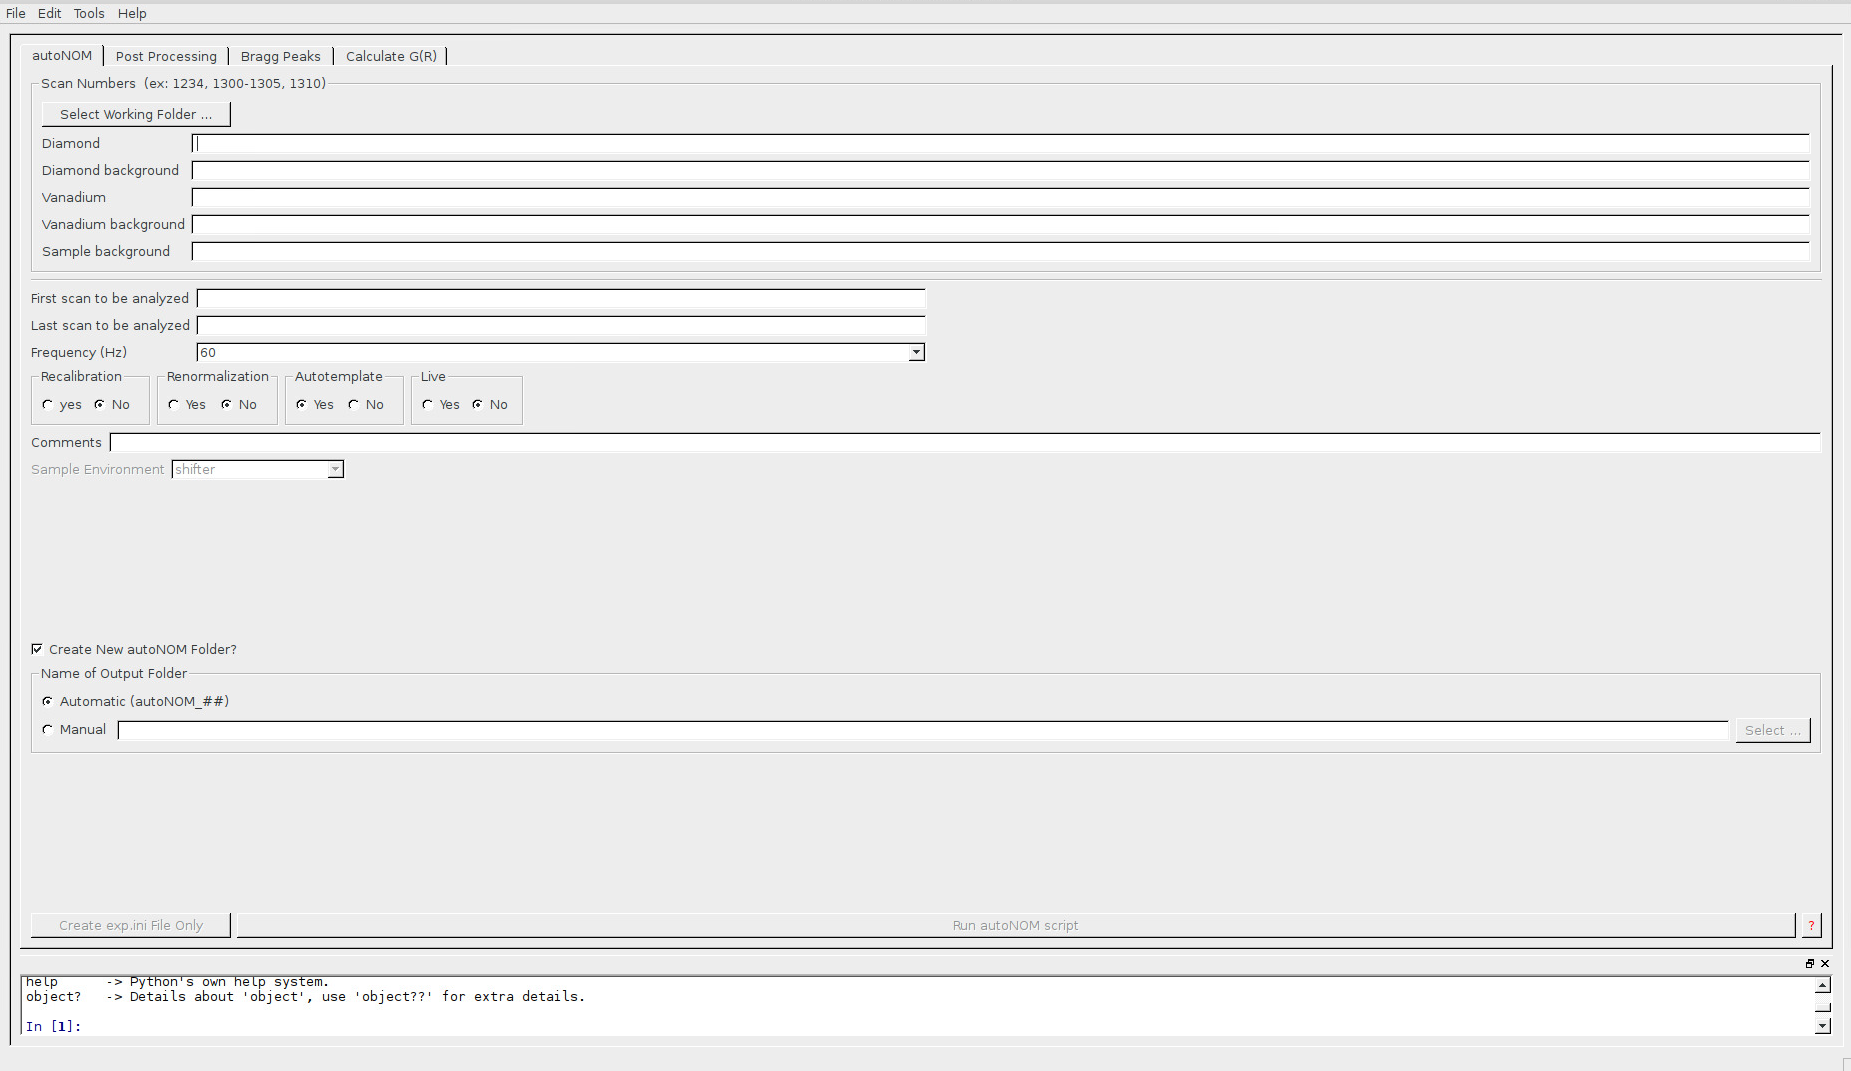
\includegraphics[width=0.9\paperwidth]{graphics/tab1/tab1.png}}

Here, we input the run numbers for the necessary measurements specified in Equation \ref{eq_intensities} in order to create our reduced data, Equation \ref{eq_reduction}. To read in this data from an experiment input file (the \fileio{exp.ini} file), click on the \guicmd{Select Working Folder...} button at the top. You will be presented with a dialog box that will prompt you to select a working directory. It will begin with your current working directory, which you can see displayed at the top in the \guicmd{Look in:} field. If you are in your \iptsPrint directory, you should get something as below:

\noindent\makebox[\textwidth]{\includegraphics[width=0.9\paperwidth]{graphics/tab1/tab1_selectWorkingFolder_sharedFolder.png}}

This is the file directory structure of your IPTS. You can see the \fileio{nexus} directory where the raw neutron event files are stored, the \fileio{adara} directory (ADARA = Accelerating Data Acquisition, Reduction, and Analysis) for automated live reduction files, and the \fileio{shared} directory, which is a User workspace for the experiment. Double-click the \fileio{shared} directory and you will see something similar to the following:

\noindent\makebox[\textwidth]{\includegraphics[width=0.9\paperwidth]{graphics/tab1/tab1_selectWorkingFolder_autoNOMfolder.png}}

Here, the \fileio{autoNOM} directory is where we will kick off the autoreduction of ADDIE. This will produce the \fileio{autoreduce} directory that you see above. This IPTS has already had the data reduction performed. If your IPTS has not yet had the data reduced, you may not see either of these directories. If the \fileio{autoNOM} directory does not exists, go to the terminal, get to the shared directory above ( \cmd{cd \iptsPrint/shared} ) and create it using the command: \cmd{mkdir autoNOM}. Once this directory exists, double-click the \fileio{autoNOM} directory. You will see something similar to the following:

 \noindent\makebox[\textwidth]{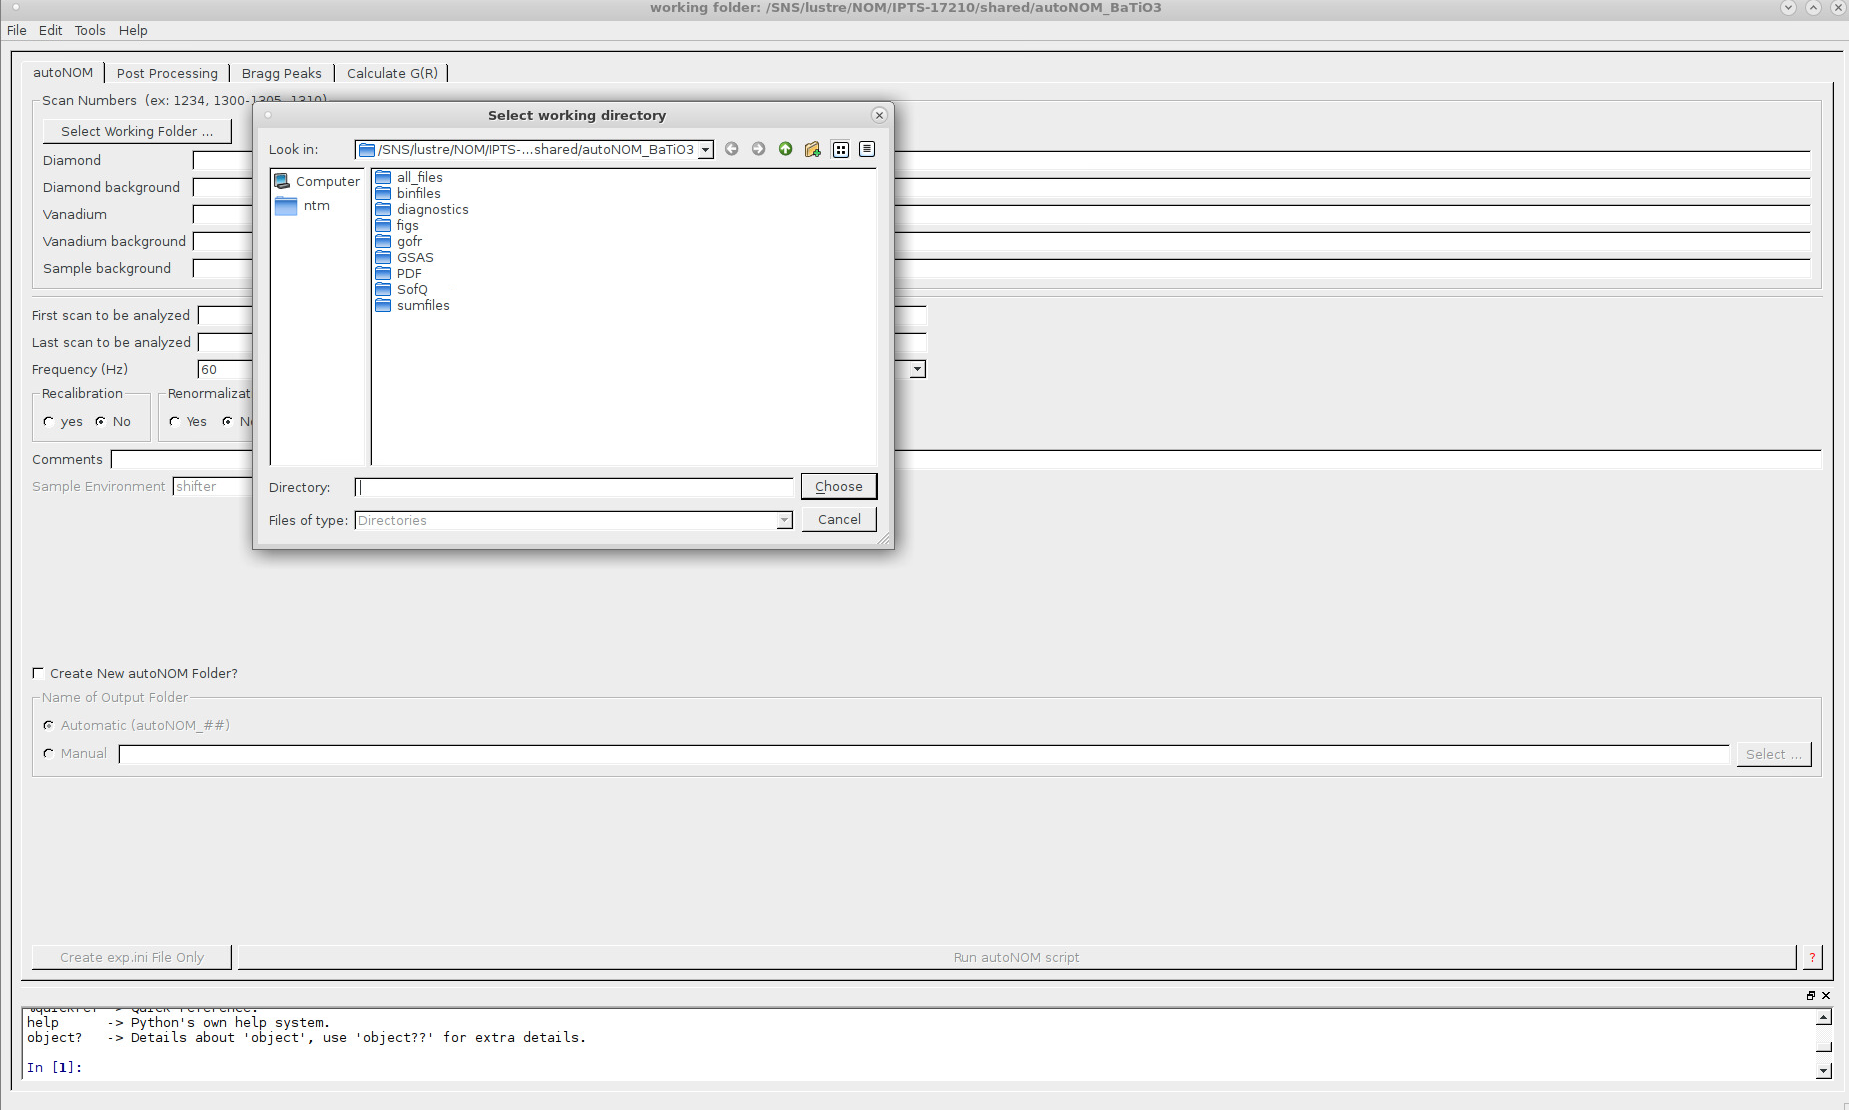
\includegraphics[width=0.9\paperwidth]{graphics/tab1/tab1_selectWorkingFolder.png}}
 
 Again, we have already launched data reduction in this IPTS so you see the directories that will be produced. For now, simply select \guicmd{Choose} on the bottom left. This will look for the experiment input file (the \fileio{exp.ini} file) in the current directory. If the file is found, the tab should populate with the experiment information in the file and look similar to the following:
 
  \noindent\makebox[\textwidth]{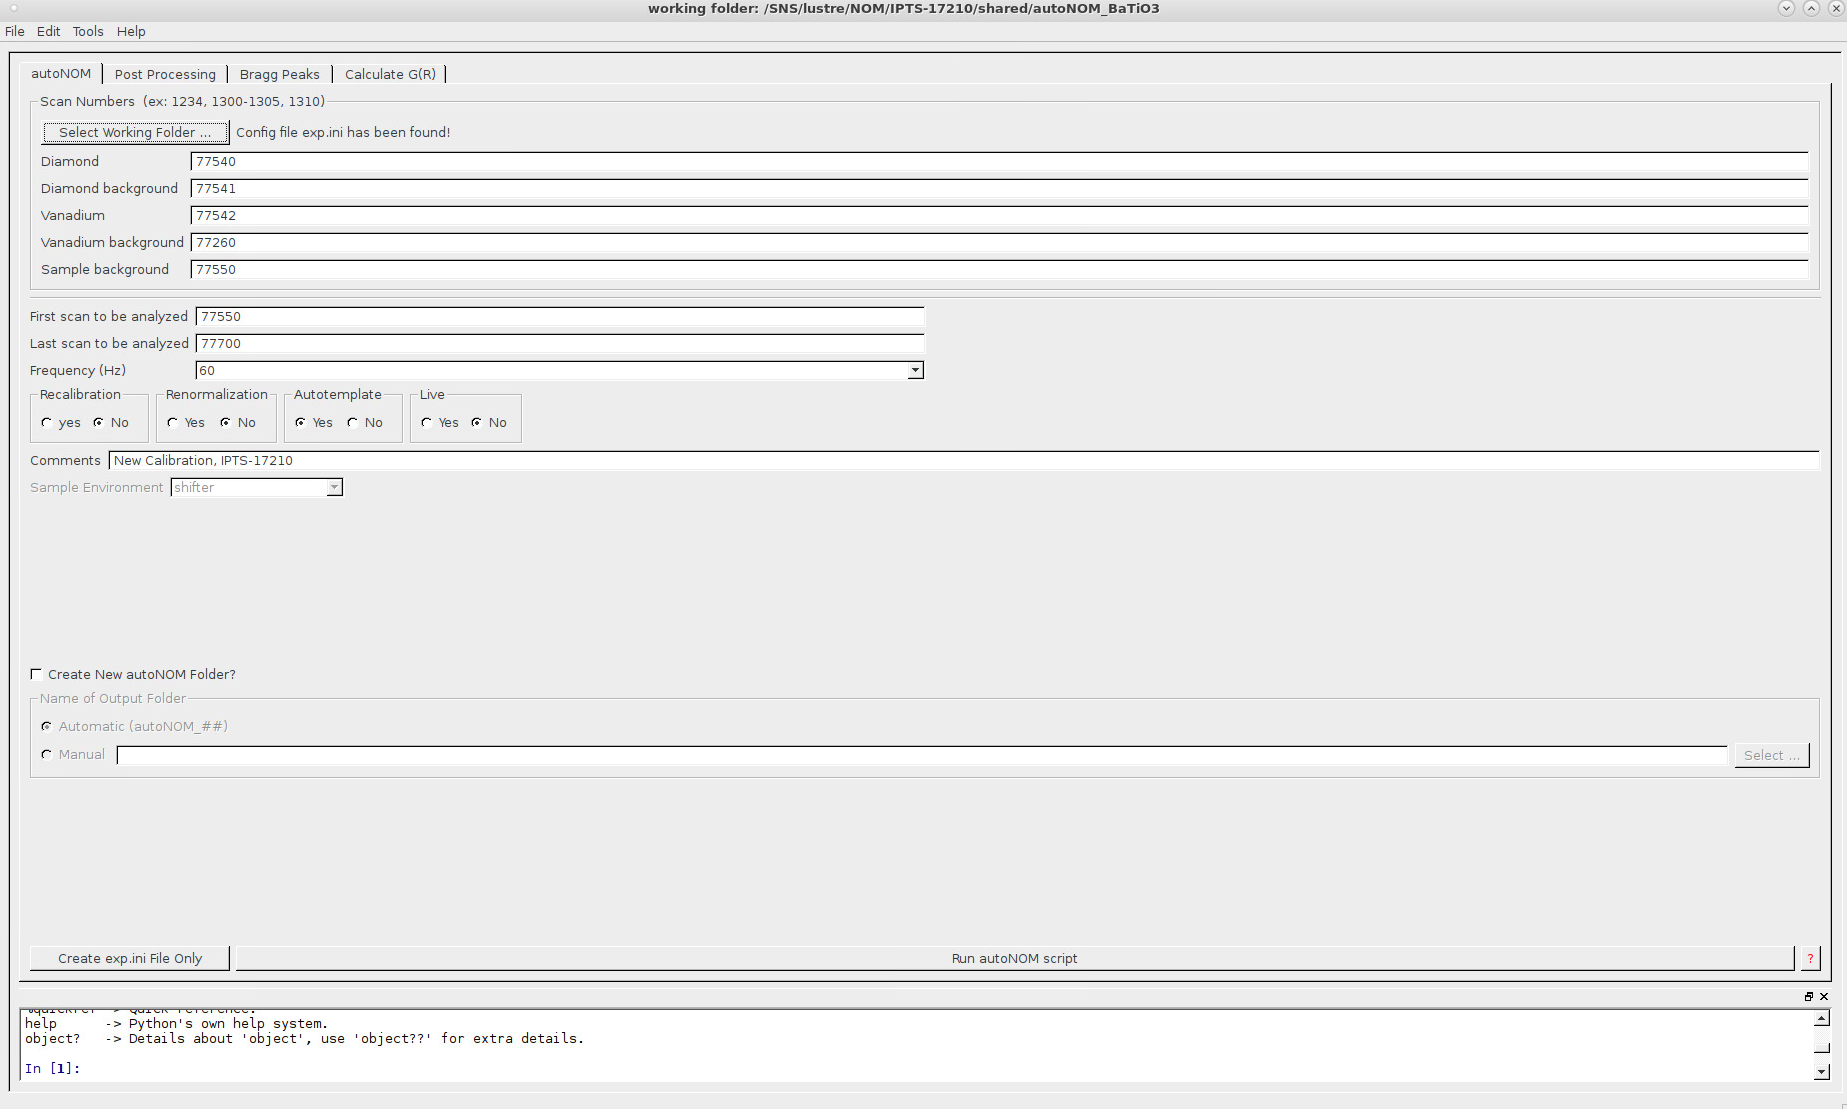
\includegraphics[width=0.9\paperwidth]{graphics/tab1/tab1_populated.png}}
  
If no experiment file was found, you will see the following next to the \guicmd{Select Working Folder...} button:

  \noindent\makebox[\textwidth]{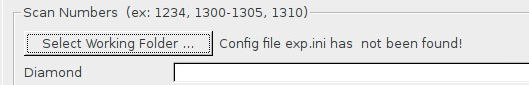
\includegraphics[width=0.5\paperwidth]{graphics/tab1/tab1_selectWorkingFolder_error.png}}
  
If this occurs, you can fill in the necessary fields. Once you have these filled in, you can output an experiment input file using the \guicmd{Create exp.ini File Only} button. Yet, this file will be automatically created once we kick off the autoreduction. 

The experiment input file (\fileio{exp.ini} file) has the following format:

  \noindent\makebox[\textwidth]{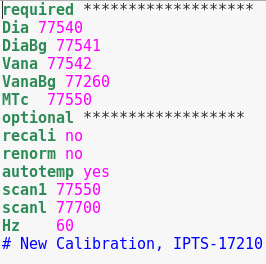
\includegraphics[width=0.25\paperwidth]{graphics/tab1/tab1_experimentInputFile.png}}

\subsubsection{If No Experiment Information File Exists}

If you do not know these run numbers required to begin processing your data but you have measured them in your current IPTS, you can create a List of Scans file (a \fileio{los.txt} file) that has this information using the following command on the command line of a terminal:

\cmd{python /SNS/NOM/shared/autoNOM/stable/readtitles.py}

You can open this file (\fileio{los.txt} from ADDIE by going to the \guicmd{File} drop-down from the \guicmd{Menu} bar and selecting the \guicmd{Preview Ascii...} and selecting the \fileio{los.txt} file. You can optionally use a text editor (\fileio{gedit, vim, emacs}) from a terminal.

  \noindent\makebox[\textwidth]{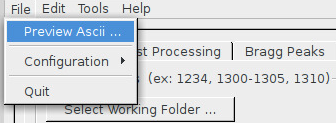
\includegraphics[width=0.3\paperwidth]{graphics/dropdown/dropdown_file_previewAscii.png}}
  
  If you have any trouble with this step, please contact your Local Instrument Scientist Contact to help you get the necessary files. These can even be located in a directory you do not have access to, in which case, the Instrument Scientist can help assist you and ensure you have all the necessary files to launch the data reduction.
  

  
\subsection{Setting up Data Reduction}

At this point, you should have experiment information input into the tab similar to the following:

  \noindent\makebox[\textwidth]{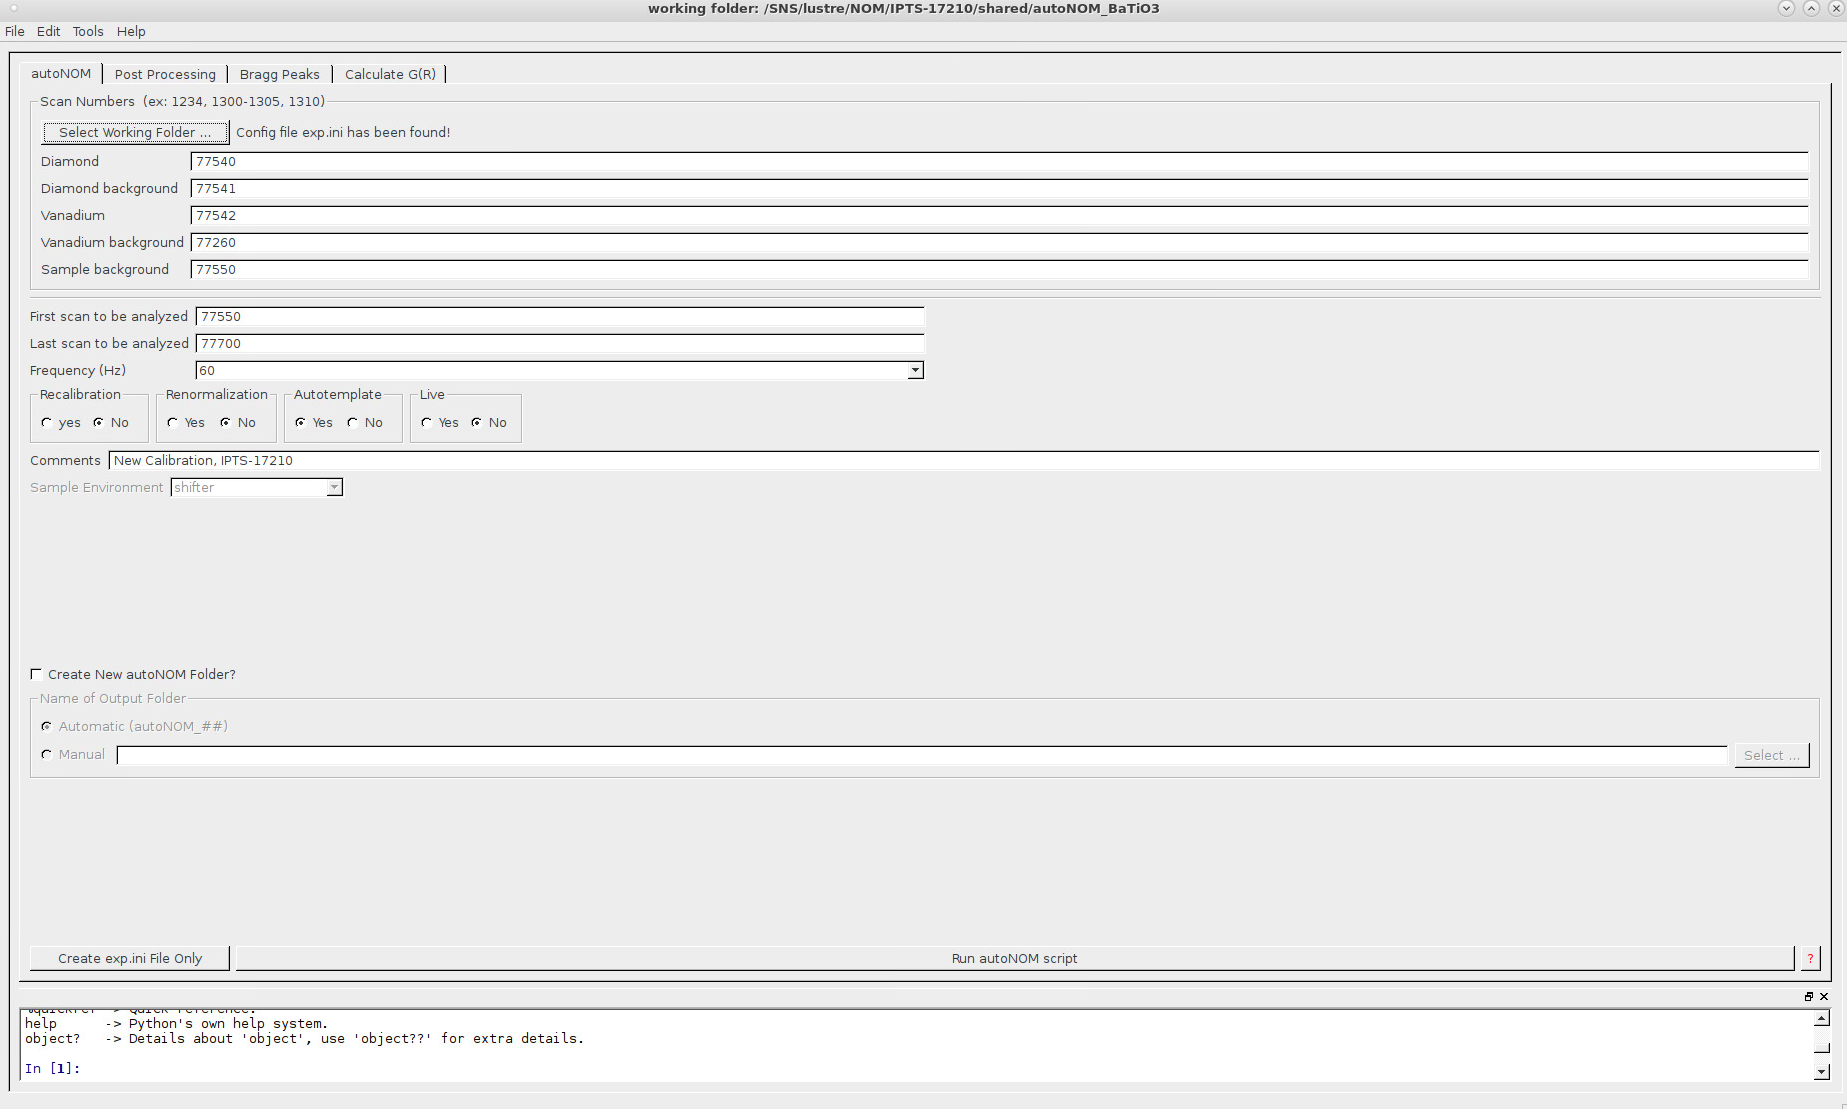
\includegraphics[width=0.9\paperwidth]{graphics/tab1/tab1_populated.png}}
  
  
If you have questions about the run numbers (Diamond, Vanadium, Backgrounds, etc.) and what they are used for, please refer to Section \ref{sec_background} for an explanation. 

Settings:
\begin{itemize}

\item \guicmd{First scan to be analyzed}: we input the first run number of your IPTS. This can be found from the DAS where you setup the experiment and are controlling the instrument. It will be under \fileio{Run Information} as \fileio{Run Number}, similar to the following where the run number is 91566:

  \noindent\makebox[\textwidth]{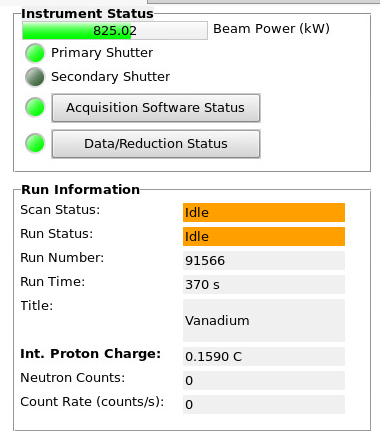
\includegraphics[width=0.25\paperwidth]{graphics/das_runInformation.png}}
  
\item \guicmd{Last scan to be analyzed}: The last run to be analyzed. If you are running a "live" experiment, you can set this to an arbitrarily large run number. Only run numbers with associated NeXus files under the current IPTS will be found and reduced. 

\item \guicmd{Frequency}: Change the frequency mode of the data reduction. You can select from either 60 Hz (use every proton pulse that hits the target) or 30 Hz (use every other proton pulse). You can use the 30 Hz mode to use longer times-of-flight and thus longer wavelenths. Typically, we operate in the 60 Hz mode. 

\item \guicmd{Recalibration}: Either use the current calibration files present or re-perform calibration using the input Diamond run. If the re-calibration is set to \fileio{No} but no calibration files are found, it will automatically perform the calibration again. 

\item \guicmd{Renormalization}:   Either use the current normalization files present or re-perform calibration using the input Vanadium run. If the re-normalization is set to \fileio{No} but no normalization files are found, it will automatically perform the normalization again. 

\item \guicmd{Autotemplate}: Setup an organized directory structure under the autoNOM parent diretory. Always recommended and preferred.

\item \guicmd{Live}: Launch data reduction in either live mode where NeXus files will continuously be produced or in a post-processing mode where data reduction will stop once the last scan is analyzed. 

\item \guicmd{Commend}: This is a place to store a metadata comment about the experiment input information. Examples would be in what IPTS were the diamond and vanadium runs used from if they did not come from this ITPS, what was the sample environment, and any other information. This will be stored in the experiment input file (the \fileio{exp.ini} file).

\item \guicmd{Sample Environment} Specifies the sample environment. Used to determine if a calibration already exists for this sampel environment.

\item \guicmd{Creaete New autoNOM Folder?}: When data reduction is launched, this will create a new autoNOM directory and work within that folder. If you have already made an autoNOM directory, uncheck this box or you will have an autoNOM directory inside another autoNOM directory. You can let the autoNOM directory be automatically named sequentially or you can manually input the name of the directory.

\end{itemize}

\subsection{Launch Data Reduction}
Once the data reduction is setup and ready, you can kick off the automatic data reduction by pressing the \guicmd{Run autoNOM script} button. If everything is okay, you should see the Job Monitor window appear with the status of the job: 

  \noindent\makebox[\textwidth]{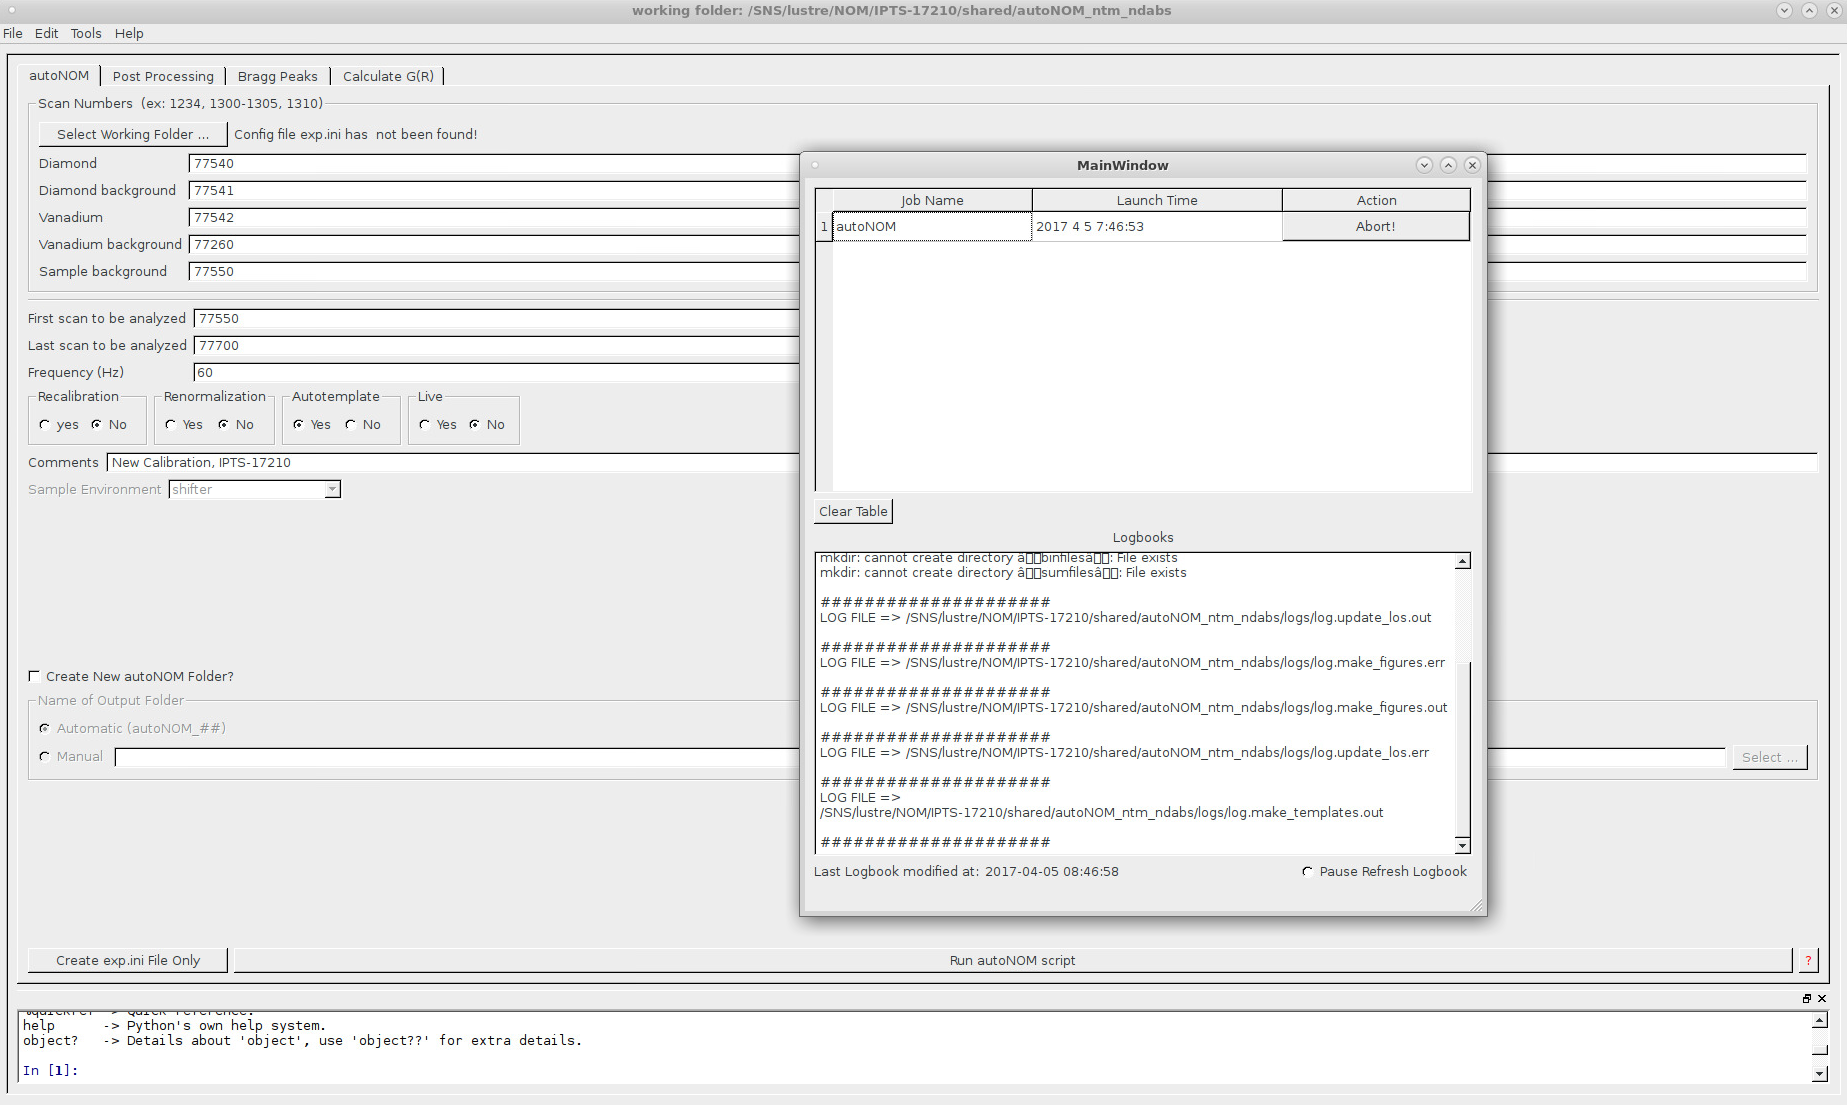
\includegraphics[width=0.3\paperwidth]{graphics/tab1/tab1_runAutoNOM_jobMonitor.png}}
  
If not running in "Live" mode, you will see a display of \guicmd{Done!} when the job is complete.

The Logbooks in the Job Monitor window display the output from log files that are saved and located in the \fileio{logs} directory under the parent autoNOM directory. Only the most recent Logbooks are displayed. The Logbook view is updated every 5 seconds by default. If you would like to pause the Logbook to scroll up and see the output, you can check the \guicmd{Pause Refresh Logbook} radio button at the bottom. Once you are done and want to refresh the Logbook, simply press the same button again to uncheck it.

If, at any time, you need to stop the data reduction, you can press the \guicmd{Abort!} button to kill all the running processes associated with the job. You will see a display of \guicmd{Killed!} when the job is finished aborting.

If the \guicmd{Run autoNOM script} button is greyed out and you cannot select it, something is missing from the data reduction setup. Press the question mark button located beside the \guicmd{Run autoNOM script} button and you will be shown what is missing in the pop-up Button Status window. Below, we have forgot the Diamond background:

  \noindent\makebox[\textwidth]{\includegraphics[width=0.3\paperwidth]{graphics/tab1/tab1_runAutoNOM_questionMark.png}}

\subsection{Getting files from another IPTS}

If the diamond, vanadium, and background runs where processed in another, you can use the IPTS File Transfer tool to move over those files and bypass the need to repeat the calibration and normalization steps. \textbf{NOTE:} On \analysis, you must have the necessary permissions to access another IPTS. This may need to be performed by an Instrument Scientist with the correct permissions. If the runs exists in another IPTS but have not been processed yet, then you can proceed as normal. If you have the necessary permissions, calibration and normalization will continue as if those files where in your IPTS.

To transfer files from another IPTS, go to the \guicmd{Tools} drop-down of the \guicmd{Menu} bar and select \guicmd{IPTS Fil Transfer...}. You will be presented with the following dialog box:

  \noindent\makebox[\textwidth]{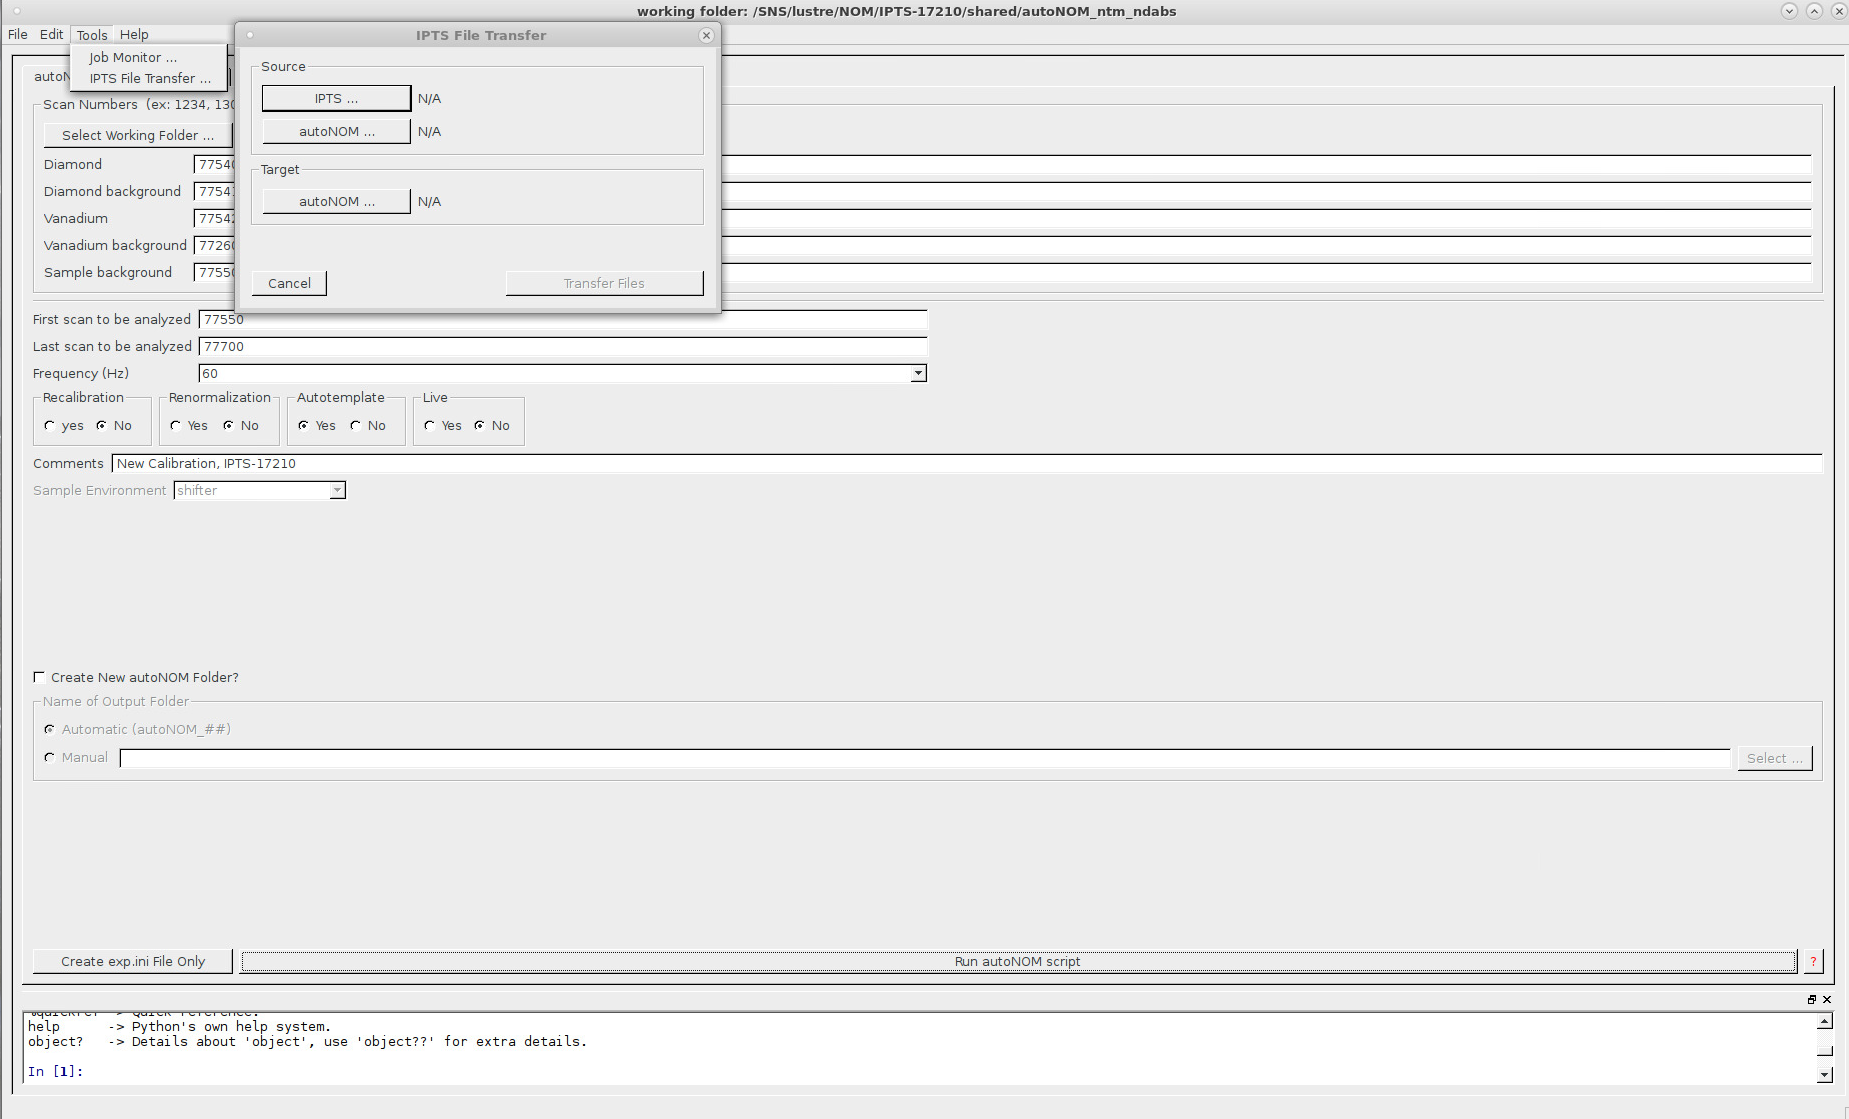
\includegraphics[width=0.3\paperwidth]{graphics/tab1/tab1_iptsFileTransfer.png}}
  
First, press the \guicmd{IPTS...} button to select the IPTS from the pop-up box. Here we are selecting IPTS-18314. Press \guicmd{Choose} once selected::

  \noindent\makebox[\textwidth]{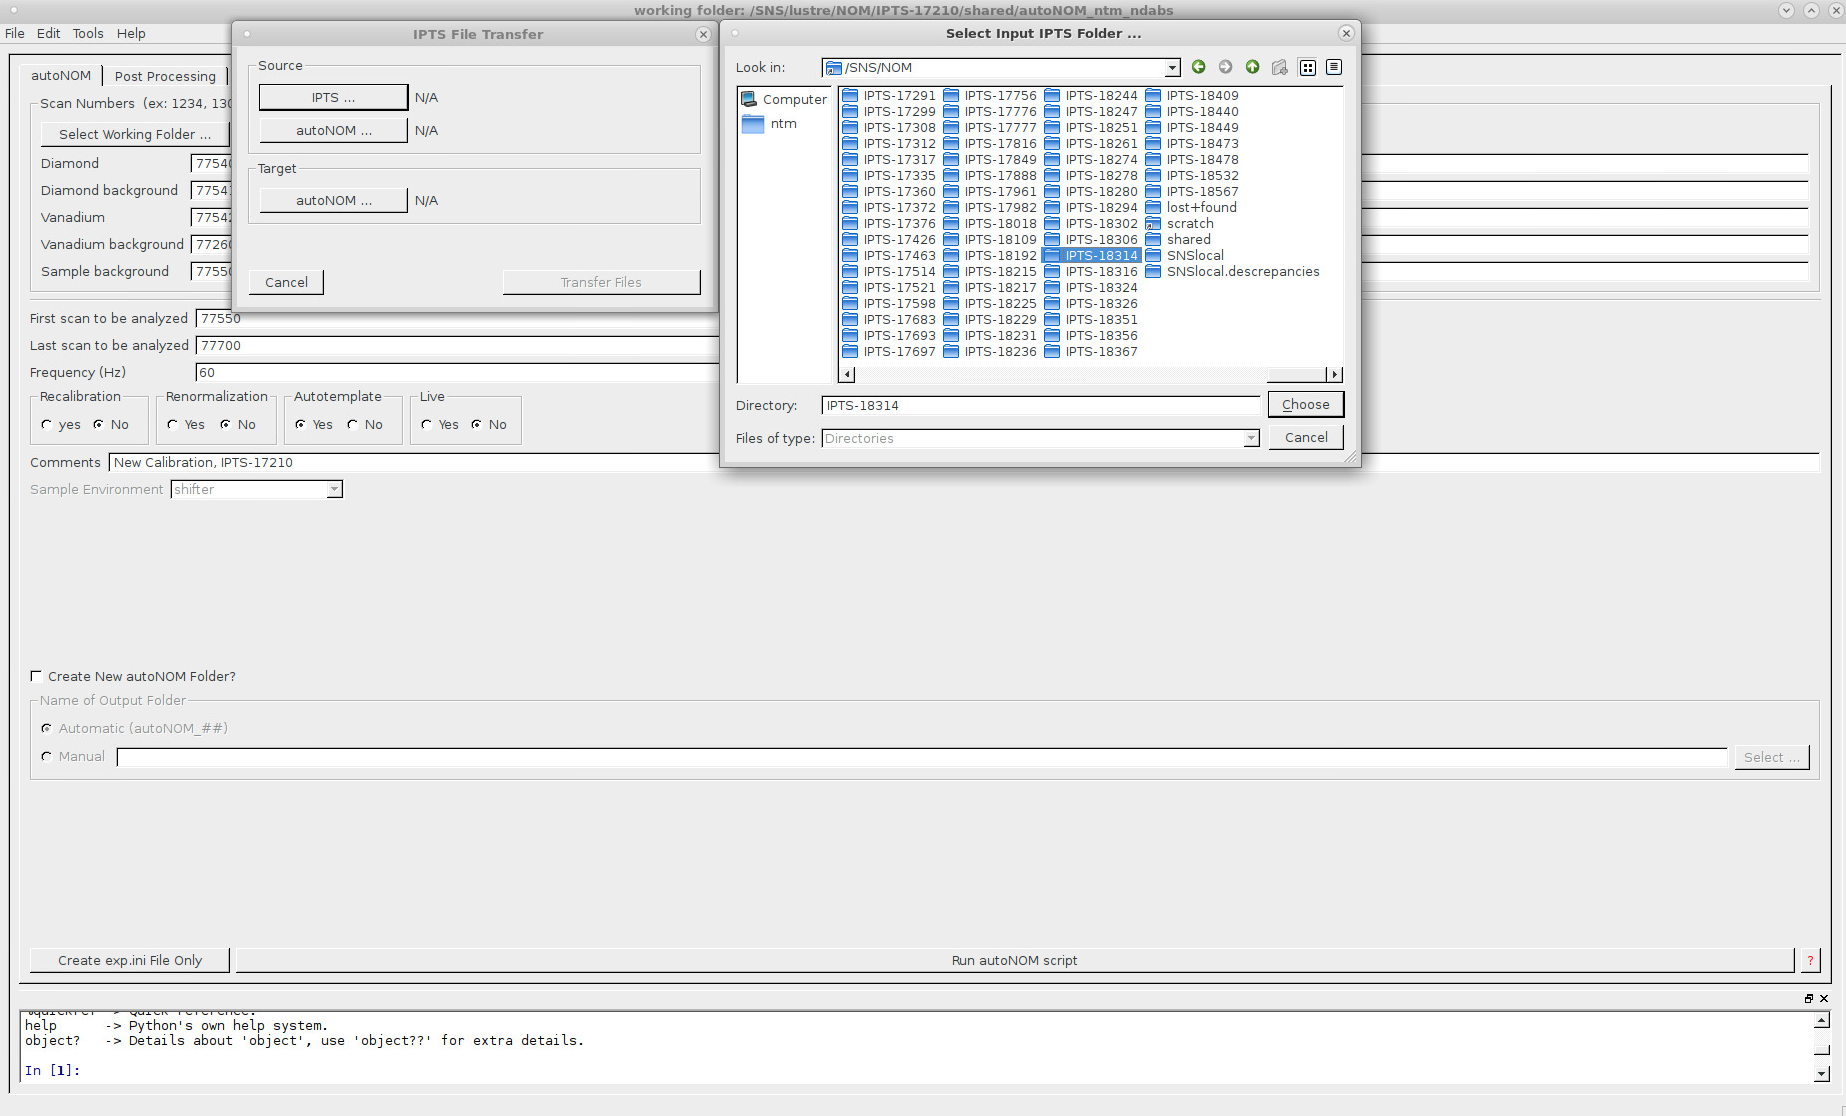
\includegraphics[width=0.3\paperwidth]{graphics/tab1/tab1_iptsFileTransfer_selectIPTS.png}}
  
  
Then, press the \guicmd{autoNOM...} button in the \textbf{Source} section to select the specific autoNOM directory. From below, you can see that an IPTS can have multiple autoNOM directories. We are selecting the autoNOM\_2017A\_cryostat below. Press \guicmd{Choose} once selected:

  \noindent\makebox[\textwidth]{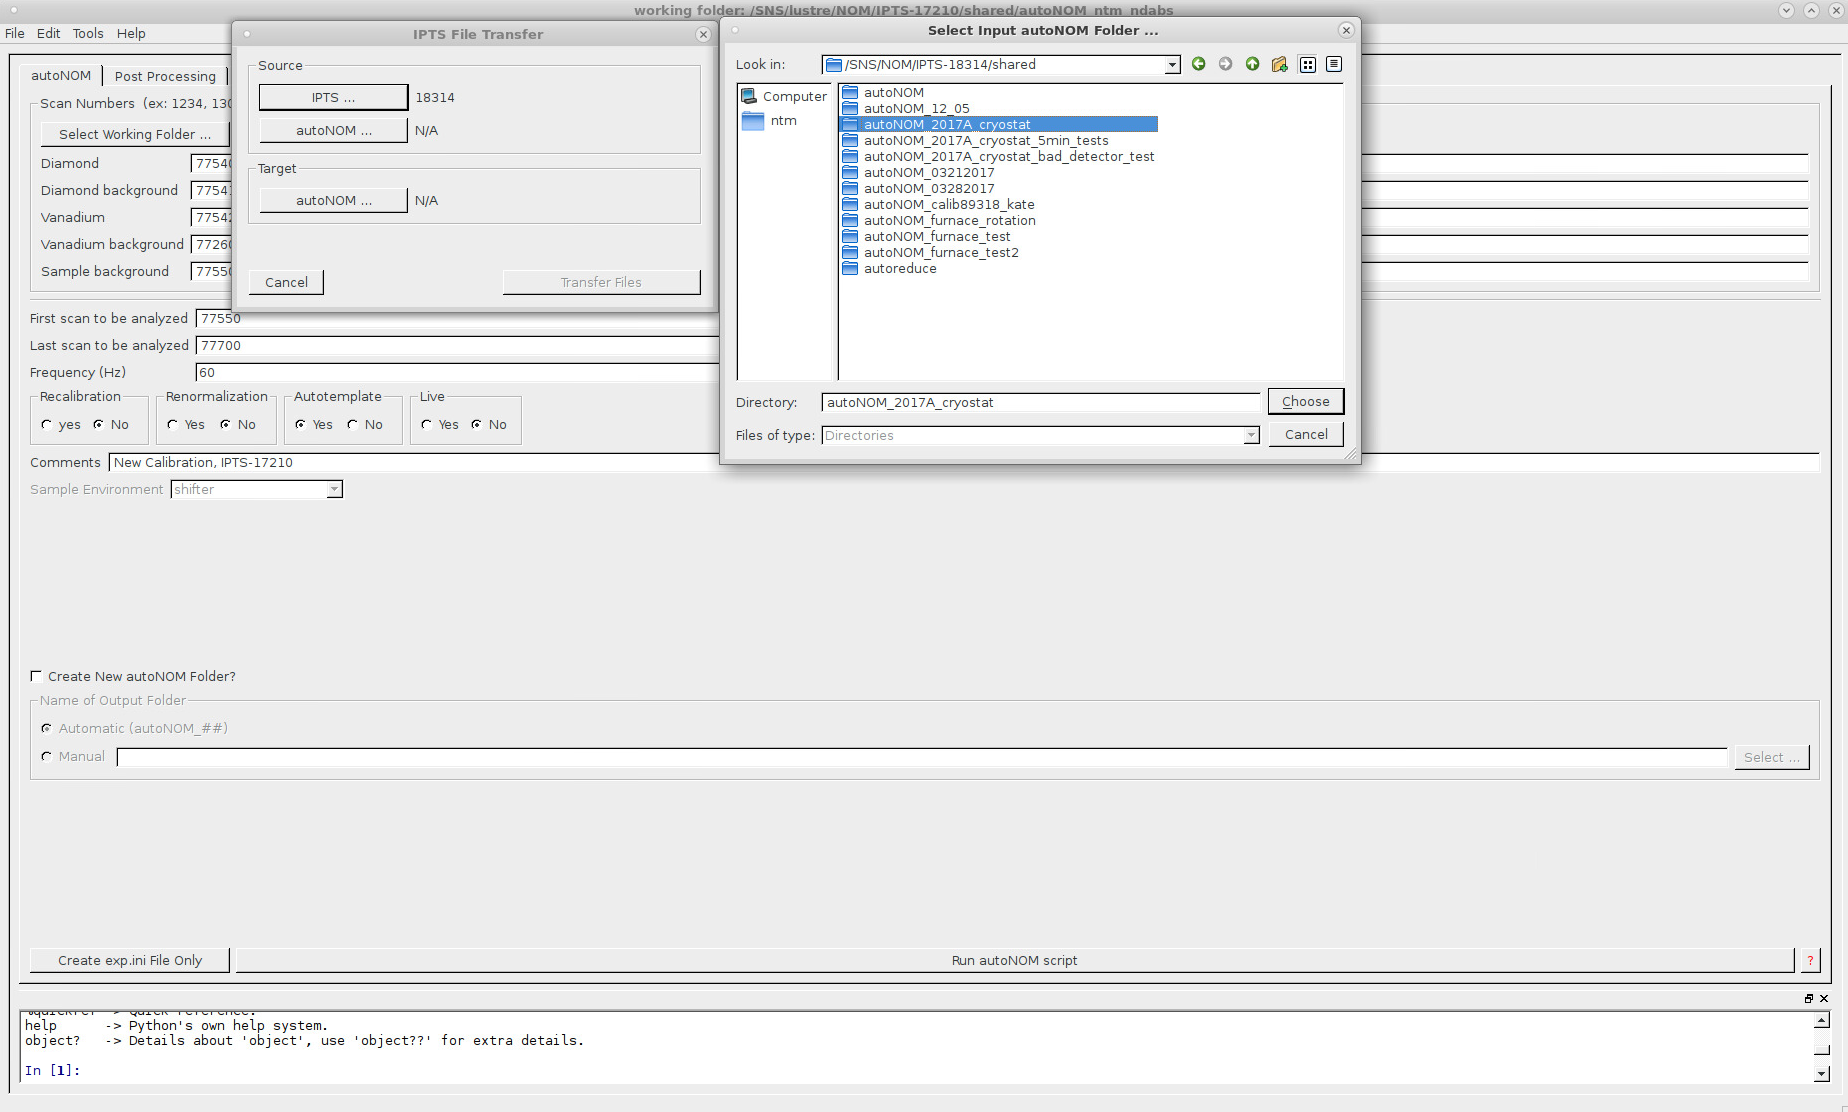
\includegraphics[width=0.3\paperwidth]{graphics/tab1/tab1_iptsFileTransfer_selectAutonomFrom.png}}
  
Finally, press the \guicmd{autoNOM...} button in the \textbf{Target} section to select where you will transfer the files. We are selecting the autoNOM\_new\_test directory below in IPTS-17210. Press \guicmd{Choose} once selected:

  \noindent\makebox[\textwidth]{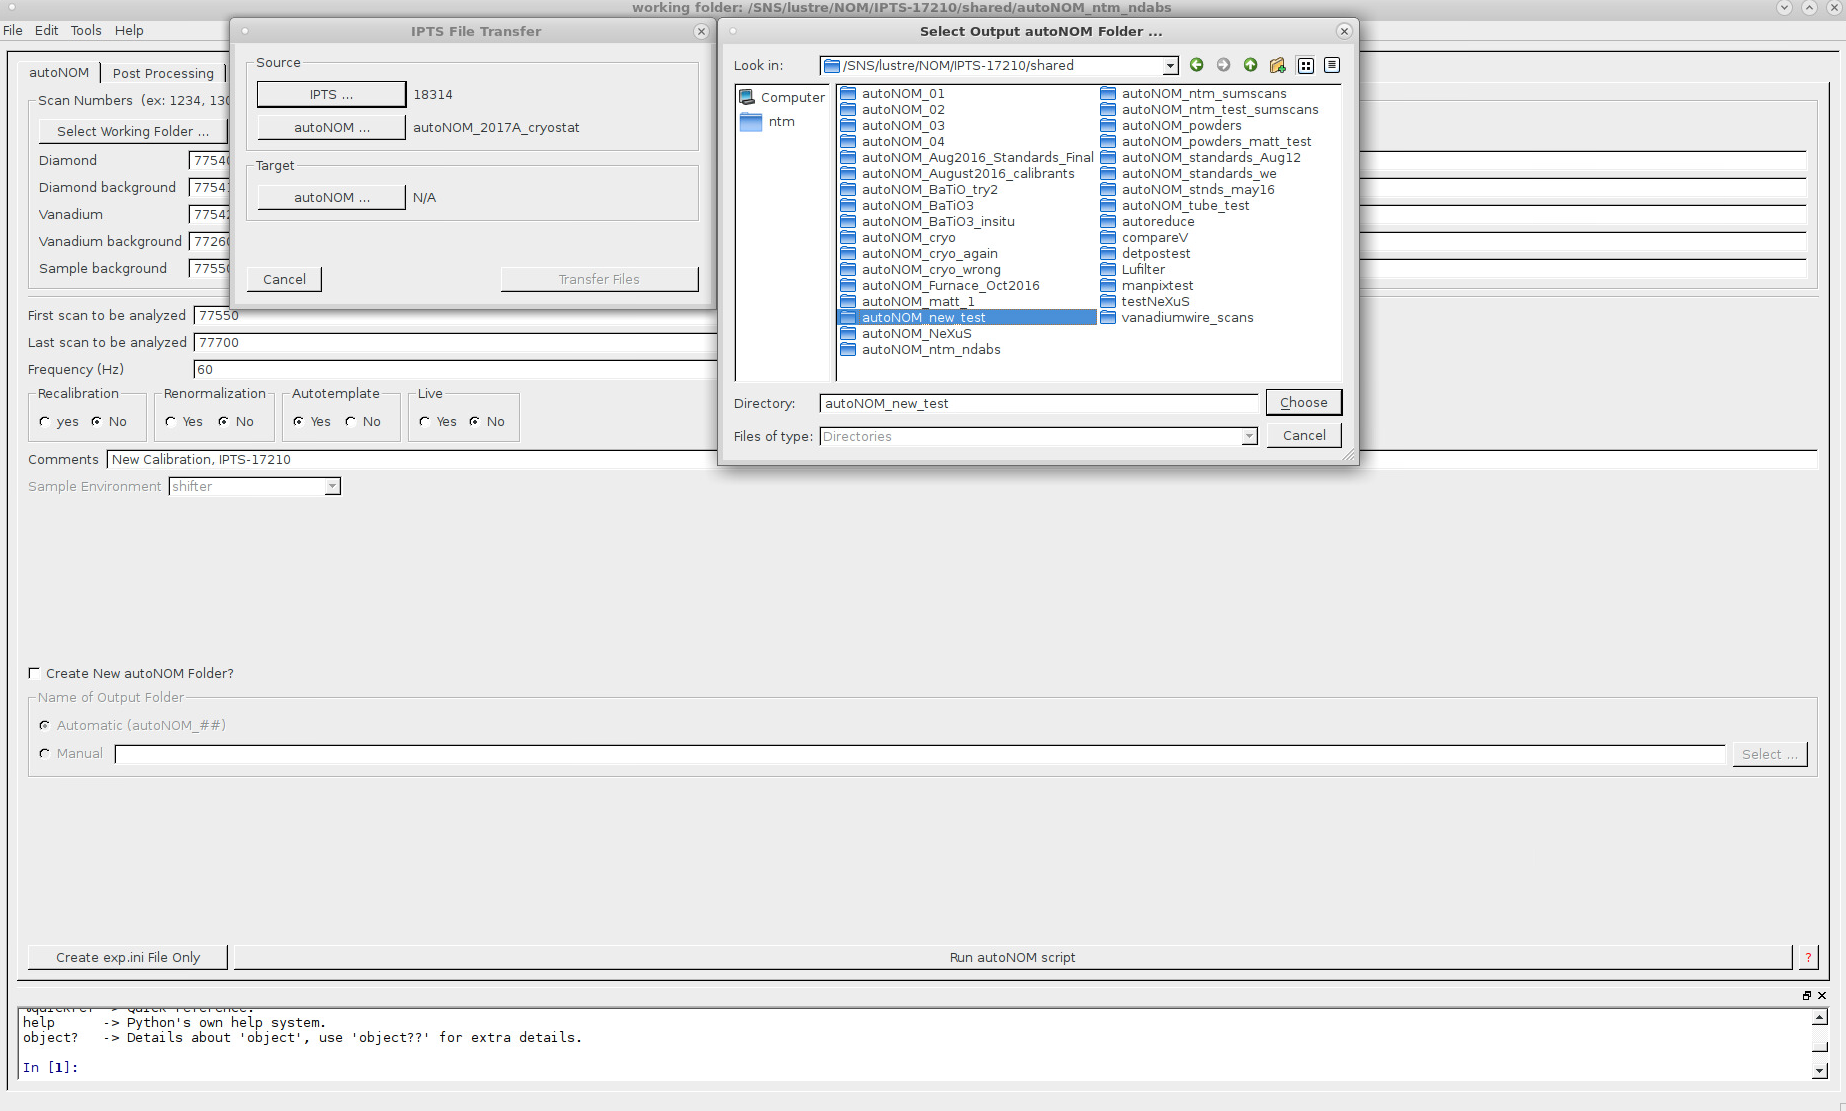
\includegraphics[width=0.3\paperwidth]{graphics/tab1/tab1_iptsFileTransfer_selectAutonomTo.png}}
  
Now, you are ready to transfer. Press the \guicmd{Transfer Files} button and the transfer will start. the Job Monitor window should appear and let you know when the transfer is complete. This is usually a very quick transfer. 

  \noindent\makebox[\textwidth]{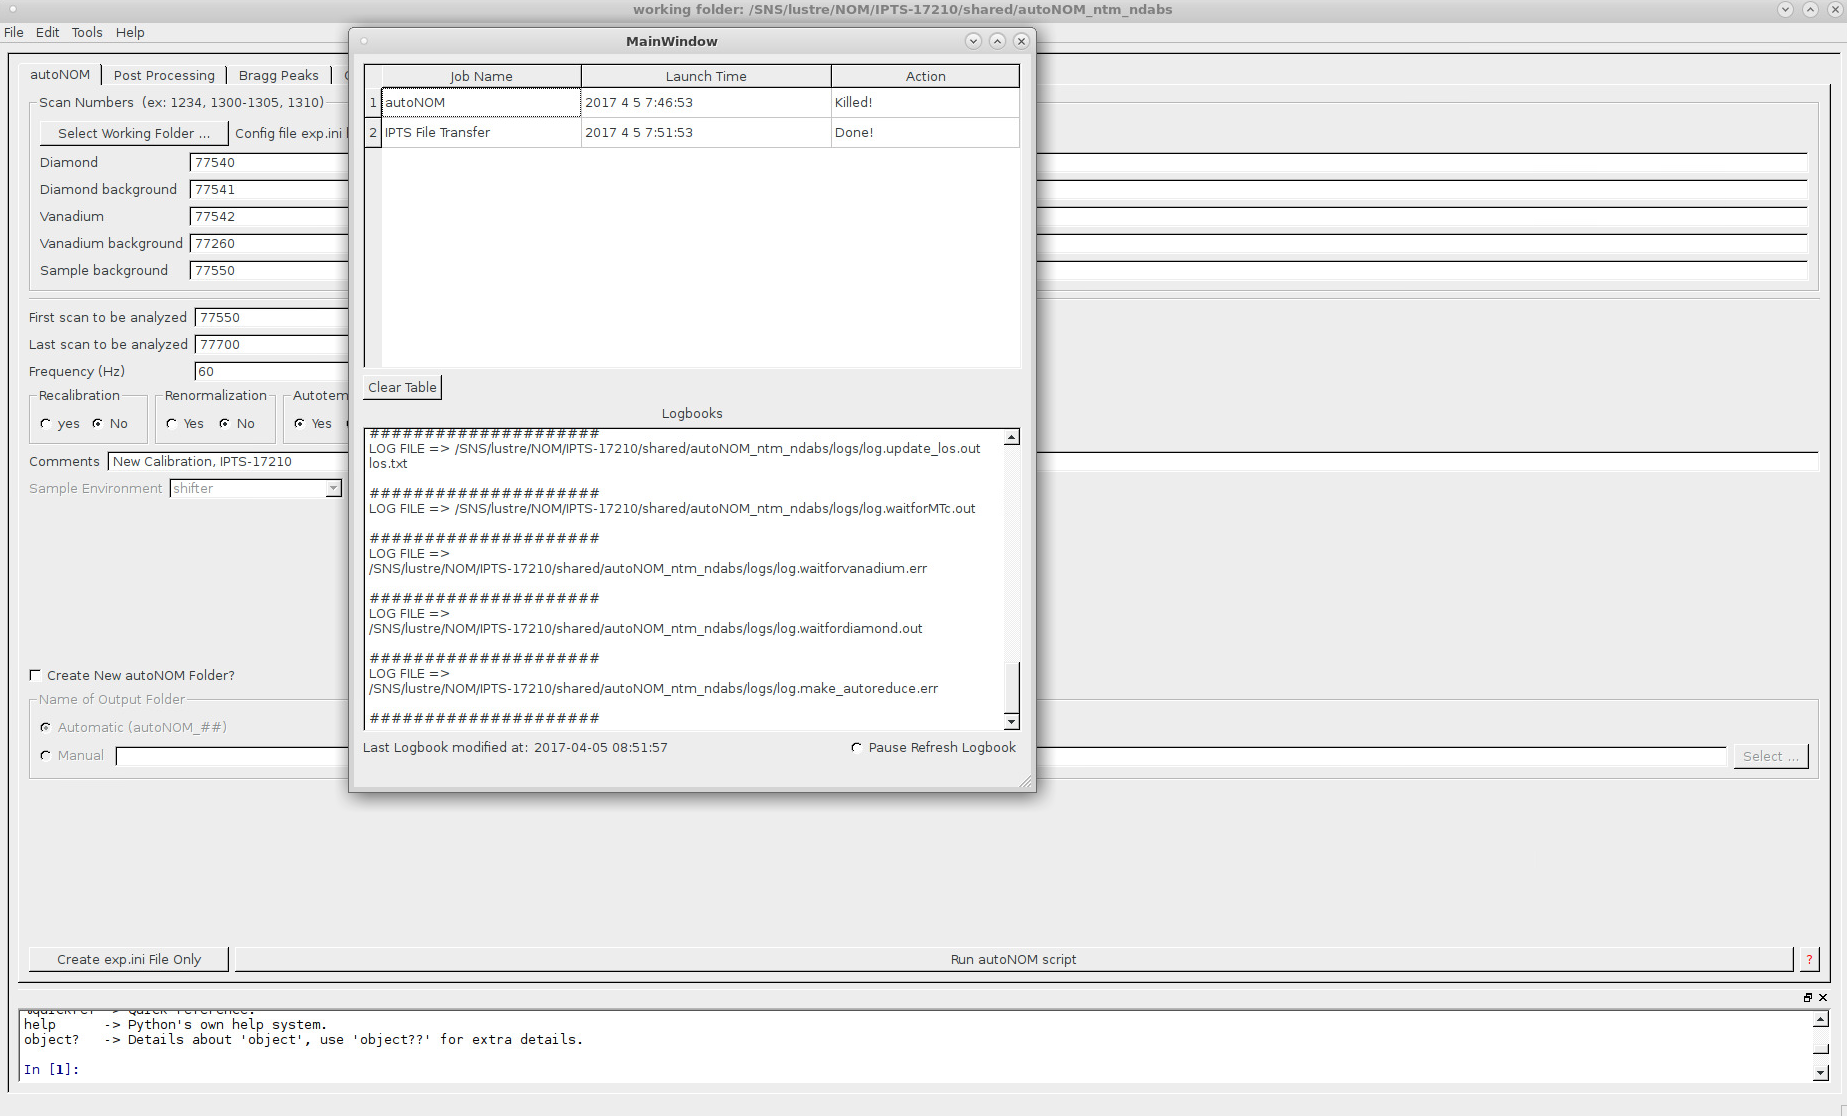
\includegraphics[width=0.3\paperwidth]{graphics/tab1/tab1_iptsFileTransfer_jobMonitor.png}}